\documentclass[14pt]{extbook}
\usepackage{multicol, enumerate, enumitem, hyperref, color, soul, setspace, parskip, fancyhdr} %General Packages
\usepackage{amssymb, amsthm, amsmath, latexsym, units, mathtools} %Math Packages
\everymath{\displaystyle} %All math in Display Style
% Packages with additional options
\usepackage[headsep=0.5cm,headheight=12pt, left=1 in,right= 1 in,top= 1 in,bottom= 1 in]{geometry}
\usepackage[usenames,dvipsnames]{xcolor}
\usepackage{dashrule}  % Package to use the command below to create lines between items
\newcommand{\litem}[1]{\item#1\hspace*{-1cm}\rule{\textwidth}{0.4pt}}
\pagestyle{fancy}
\lhead{Makeup Progress Quiz 2}
\chead{}
\rhead{Version B}
\lfoot{2790-1423}
\cfoot{}
\rfoot{Summer C 2021}
\begin{document}

\begin{enumerate}
\litem{
Choose the equation of the function graphed below.
\begin{center}
    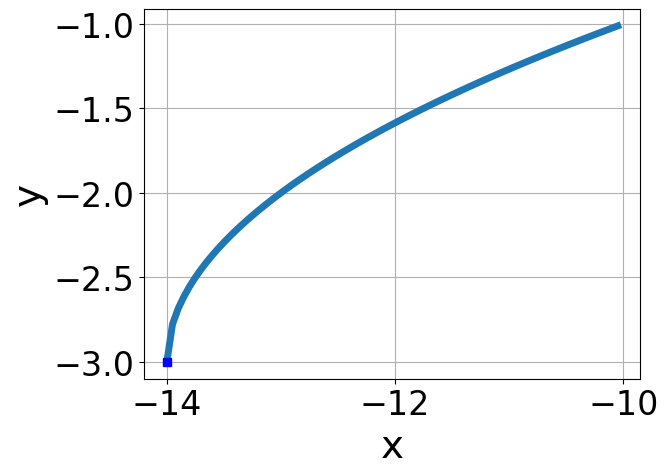
\includegraphics[width=0.5\textwidth]{../Figures/radicalGraphToEquationCopyB.png}
\end{center}
\begin{enumerate}[label=\Alph*.]
\item \( f(x) = - \sqrt[3]{x + 14} - 3 \)
\item \( f(x) = \sqrt[3]{x - 14} - 3 \)
\item \( f(x) = \sqrt[3]{x + 14} - 3 \)
\item \( f(x) = - \sqrt[3]{x - 14} - 3 \)
\item \( \text{None of the above} \)

\end{enumerate} }
\litem{
What is the domain of the function below?\[ f(x) = \sqrt[5]{5 x - 9} \]\begin{enumerate}[label=\Alph*.]
\item \( \text{The domain is } [a, \infty), \text{   where } a \in [1.8, 5.8] \)
\item \( (-\infty, \infty) \)
\item \( \text{The domain is } (-\infty, a], \text{   where } a \in [1.21, 3.04] \)
\item \( \text{The domain is } (-\infty, a], \text{   where } a \in [-0.45, 1.48] \)
\item \( \text{The domain is } [a, \infty), \text{   where } a \in [-0.44, 1.56] \)

\end{enumerate} }
\litem{
Solve the radical equation below. Then, choose the interval(s) that the solution(s) belongs to.\[ \sqrt{-54 x^2 - 12} - \sqrt{-66 x} = 0 \]\begin{enumerate}[label=\Alph*.]
\item \( x \in [0.43,1.19] \)
\item \( \text{All solutions lead to invalid or complex values in the equation.} \)
\item \( x_1 \in [-1.42, -0.22] \text{ and } x_2 \in [-7,-0] \)
\item \( x \in [-0.1,0.86] \)
\item \( x_1 \in [-0.1, 0.86] \text{ and } x_2 \in [1,3] \)

\end{enumerate} }
\litem{
Choose the graph of the equation below.\[ f(x) = \sqrt{x - 10} + 3 \]\begin{enumerate}[label=\Alph*.]
\begin{multicols}{2}\item 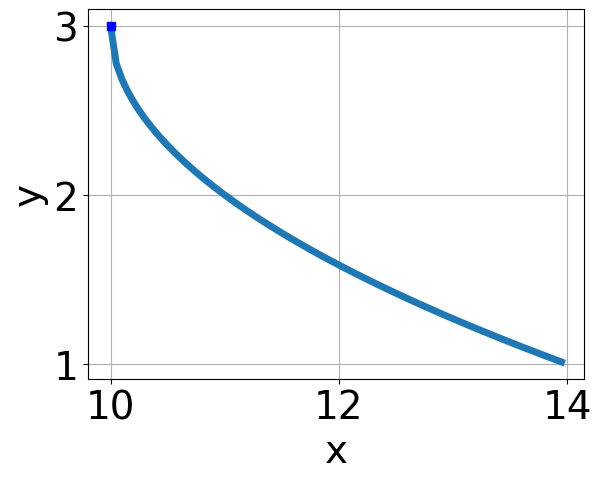
\includegraphics[width = 0.3\textwidth]{../Figures/radicalEquationToGraphAB.png}\item 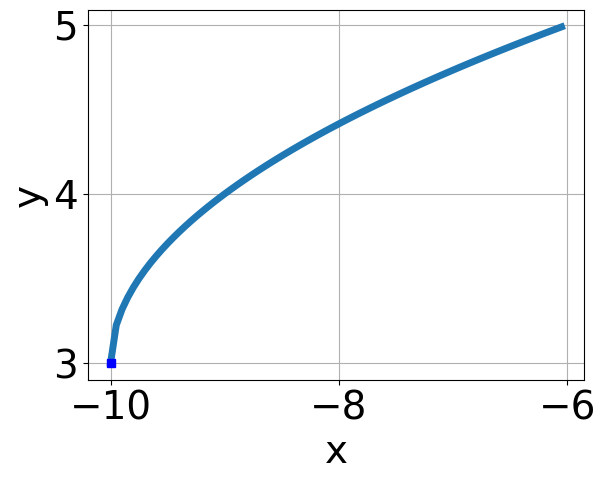
\includegraphics[width = 0.3\textwidth]{../Figures/radicalEquationToGraphBB.png}\item 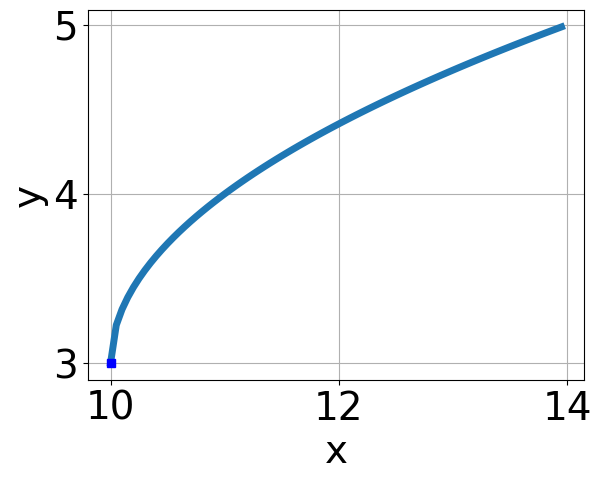
\includegraphics[width = 0.3\textwidth]{../Figures/radicalEquationToGraphCB.png}\item 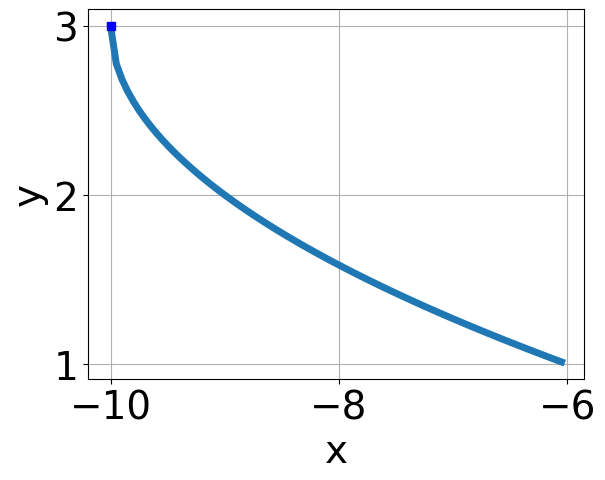
\includegraphics[width = 0.3\textwidth]{../Figures/radicalEquationToGraphDB.png}\end{multicols}\item None of the above.
\end{enumerate} }
\litem{
What is the domain of the function below?\[ f(x) = \sqrt[3]{8 x + 6} \]\begin{enumerate}[label=\Alph*.]
\item \( \text{The domain is } [a, \infty), \text{   where } a \in [-0.88, -0.52] \)
\item \( (-\infty, \infty) \)
\item \( \text{The domain is } (-\infty, a], \text{   where } a \in [-1.02, 0.07] \)
\item \( \text{The domain is } (-\infty, a], \text{   where } a \in [-1.55, -1.18] \)
\item \( \text{The domain is } [a, \infty), \text{   where } a \in [-1.5, -1.13] \)

\end{enumerate} }
\litem{
Solve the radical equation below. Then, choose the interval(s) that the solution(s) belongs to.\[ \sqrt{9 x - 7} - \sqrt{2 x - 4} = 0 \]\begin{enumerate}[label=\Alph*.]
\item \( \text{All solutions lead to invalid or complex values in the equation.} \)
\item \( x_1 \in [0.24, 0.69] \text{ and } x_2 \in [-0.9,1.1] \)
\item \( x_1 \in [0.46, 1.06] \text{ and } x_2 \in [1.4,3.6] \)
\item \( x \in [0.24,0.69] \)
\item \( x \in [1.33,1.59] \)

\end{enumerate} }
\litem{
Choose the equation of the function graphed below.
\begin{center}
    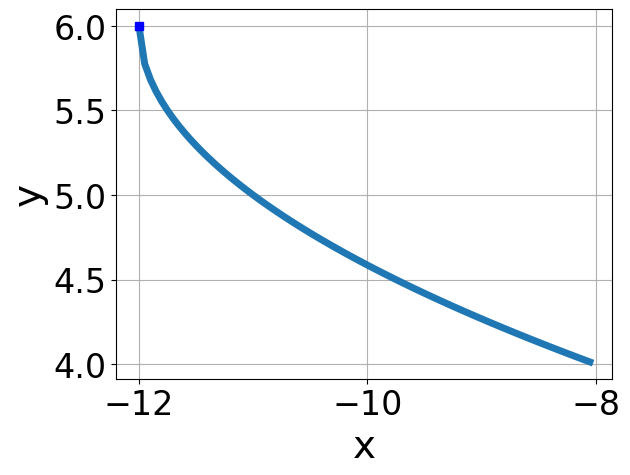
\includegraphics[width=0.5\textwidth]{../Figures/radicalGraphToEquationB.png}
\end{center}
\begin{enumerate}[label=\Alph*.]
\item \( f(x) = - \sqrt[3]{x + 12} + 6 \)
\item \( f(x) = \sqrt[3]{x - 12} + 6 \)
\item \( f(x) = - \sqrt[3]{x - 12} + 6 \)
\item \( f(x) = \sqrt[3]{x + 12} + 6 \)
\item \( \text{None of the above} \)

\end{enumerate} }
\litem{
Solve the radical equation below. Then, choose the interval(s) that the solution(s) belongs to.\[ \sqrt{63 x^2 + 10} - \sqrt{59 x} = 0 \]\begin{enumerate}[label=\Alph*.]
\item \( x_1 \in [0.13, 0.45] \text{ and } x_2 \in [0.45,1.13] \)
\item \( x_1 \in [-1.01, -0.69] \text{ and } x_2 \in [-0.77,-0.07] \)
\item \( x \in [0.64,1.16] \)
\item \( x \in [0.13,0.45] \)
\item \( \text{All solutions lead to invalid or complex values in the equation.} \)

\end{enumerate} }
\litem{
Choose the graph of the equation below.\[ f(x) = - \sqrt{x - 12} + 7 \]\begin{enumerate}[label=\Alph*.]
\begin{multicols}{2}\item 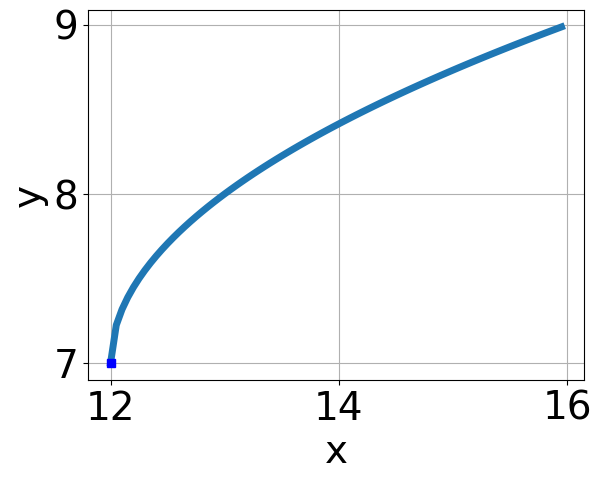
\includegraphics[width = 0.3\textwidth]{../Figures/radicalEquationToGraphCopyAB.png}\item 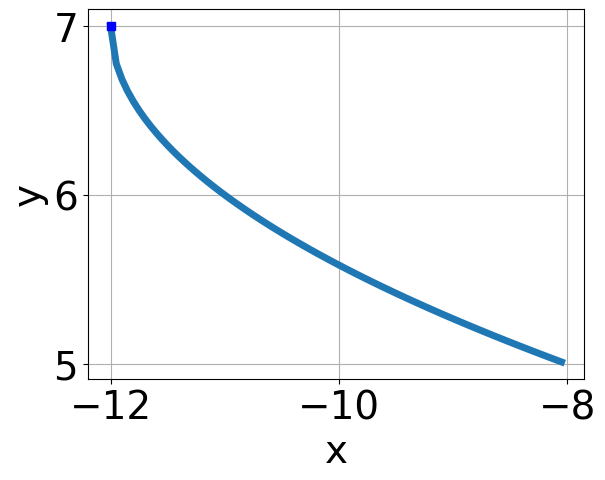
\includegraphics[width = 0.3\textwidth]{../Figures/radicalEquationToGraphCopyBB.png}\item 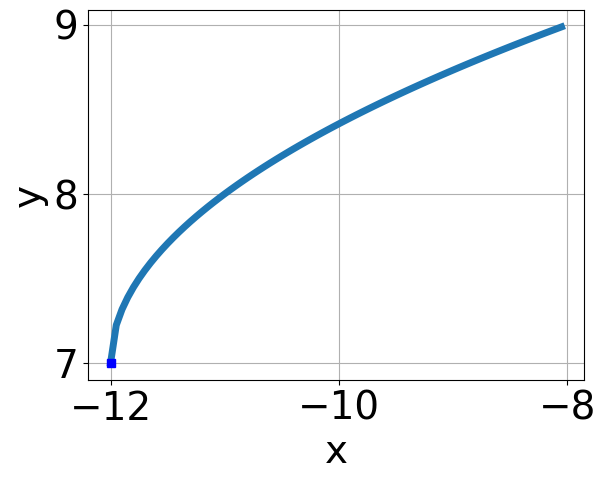
\includegraphics[width = 0.3\textwidth]{../Figures/radicalEquationToGraphCopyCB.png}\item 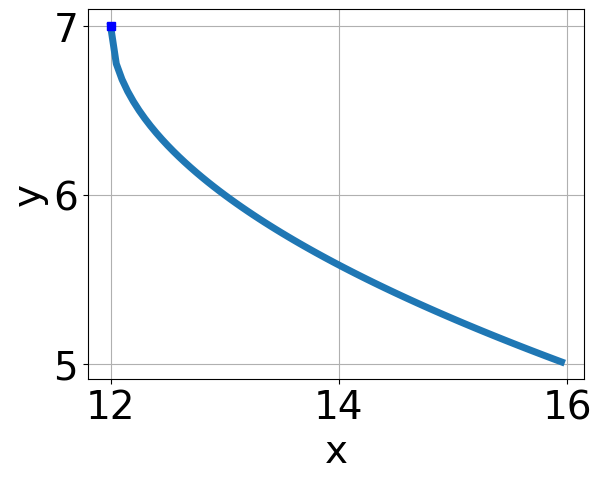
\includegraphics[width = 0.3\textwidth]{../Figures/radicalEquationToGraphCopyDB.png}\end{multicols}\item None of the above.
\end{enumerate} }
\litem{
Solve the radical equation below. Then, choose the interval(s) that the solution(s) belongs to.\[ \sqrt{-9 x - 4} - \sqrt{-3 x - 5} = 0 \]\begin{enumerate}[label=\Alph*.]
\item \( \text{All solutions lead to invalid or complex values in the equation.} \)
\item \( x \in [-0.05,0.3] \)
\item \( x_1 \in [-1.93, -1.61] \text{ and } x_2 \in [-1.59,-0.14] \)
\item \( x_1 \in [-0.71, -0.36] \text{ and } x_2 \in [0.11,0.78] \)
\item \( x \in [-1.61,-1.25] \)

\end{enumerate} }
\end{enumerate}

\end{document}